\documentclass{article}
\usepackage[utf8]{inputenc}
\usepackage[english]{babel}
\usepackage [autostyle, english = american]{csquotes}
\MakeOuterQuote{"}
\usepackage{graphicx}
\usepackage{enumerate}
\usepackage{float}
\graphicspath{ {} }
\usepackage{mathtools}
\usepackage{amsmath, amsthm, amssymb, amsfonts}
\usepackage{caption}
\usepackage{bm}
\usepackage{fancyhdr}
\pagestyle{fancy}
\fancyhf{}
\rhead{Ty Darnell}
\lhead{Homework 9}

% For derivatives
\newcommand{\deriv}[1]{\frac{\mathrm{d}}{\mathrm{d}x} (#1)}

% For partial derivatives
\newcommand{\pderiv}[2]{\frac{\partial #1}{\partial #2}}

% Integral dx
\newcommand{\dx}{\mathrm{d}x}
\newcommand{\cd}{\overset{d}{\to}}
\newcommand{\cp}{\overset{p}{\to}}
\newcommand{\B}{\beta}
\newcommand{\e}{\epsilon}
\newcommand{\limn}{\lim_{n\to \infty}}
\newcommand{\lm}{\lambda}
\newcommand{\sg}{\sigma}
\newcommand{\hb}{\hat{\beta}}
\newcommand{\sumn}{\sum_{i=1}^{n}}
\newcommand{\hth}{\hat{\theta}}
\newcommand{\lra}{\Leftrightarrow}
\newcommand{\prodn}{\prod_{i=1}^{n}}
\newcommand{\dll}[1]{\dfrac{\partial\ell}{\partial{#1}}}
\newcommand{\mle}{\hat{\theta}_{MLE}}
\newcommand{\mm}{\hat{\theta}_{MM}}
\newcommand{\sumx}{\sum_{i=1}^{n}x_i}
\newcommand{\ta}{\theta}
\newcommand{\qe}{ \ ?\ }
\newcommand{\dt}{\pderiv{}{\ta}}
\newcommand{\lt}[1]{\log(f(#1|\ta))}
\newcommand{\lx}{\lambda(x)}
\newcommand{\samp}{X_1,\dots,X_n \sim}
\newcommand{\te}{\theta_1}
\newcommand{\xm}{x_{(1)}}
\newcommand{\sn}{(\sg^2)}
\allowdisplaybreaks
\begin{document}
\begin{flushleft}

	\section*{Problem 1}
	
\begin{enumerate}[(a)]
	
	\item 
\begin{multline*}\\
n=1,4,16,64,100 \quad \alpha=.05\\
X\sim N(\mu,\sg^2) \quad(\sg^2\text{ known)}\\
H_0:\mu\leq 0 \text{ vs } H_1:\mu>0\\
L(\ta|x)=\prodn(2\pi \sg^2)^{-1/2} \exp\left(-\dfrac{(x-\mu)^2}{2\sg^2} \right)\\
=(2\pi \sg^2)^{-n/2}\exp\left(-\dfrac{\sumn(x-\mu)^2}{2\sg^2} \right)\\
\lx=\dfrac{(2\pi \sg^2)^{-n/2}\exp\left(-\dfrac{\sumn(x-\mu_0)^2}{2\sg^2} \right)}{(2\pi \sg^2)^{-n/2}\exp\left(-\dfrac{\sumn(x-\bar{x})^2}{2\sg^2} \right)}\\
=\exp\left(\left[-\sumn(x_i-\mu_0)^2+\sumn(x_i-\bar{x})^2 \right]/2\sg^2\right)\\
R=\{x:\exp\left(-n(\bar{x}-\mu_0)^2/(2\sg^2)\right)\leq c\}\\
R=\{x:(\bar{x}-\mu_0)^2\geq\dfrac{-2\sg^2\log(c)}{n} \}\\
R=\{x:|\bar{x}-\mu_0|\geq\sqrt{-\dfrac{2\sg^2\log(c)}{n}} \}\\
R=\{x:|\bar{x}-\mu_0|\geq \dfrac{\sg}{\sqrt{n}}\sqrt{-2\log(c)} \}\\
\lra
R=\{x:\dfrac{\bar{x}-\mu_0}{\sg/\sqrt{n}}\geq \sqrt{-2\log(c)} \text{ or } \leq -\sqrt{-2\log(c)} \}\\
c_1^*=\sqrt{-2\log(c)} \quad c_2^*=-\sqrt{-2\log(c)}\\
R=\{x:\dfrac{\bar{x}-\mu_0}{\sg/\sqrt{n}}\geq c_1^* \text{ or } \leq c_2^* \}\\
R=\{x:\dfrac{\bar{X}-\mu_0}{\sg/\sqrt{n}}\geq c_1^* \} \text{ (follows direction of } H_1)\\
\alpha=.05=P\left(\dfrac{\bar{X}-\mu_0}{\sg/\sqrt{n}}\geq c_1^*\right)\\
.05=P(Z>c_1^*) \quad Z\sim N(0,1)\\
.05=1-P(Z\leq c_1^*)\\
P(Z\leq c_1^*)=.95\\
qnorm(.95)=c_1^*=1.645\\
\B(\mu)=P\left(\dfrac{\bar{X}-\mu_0}{\sg/\sqrt{n}}>c_1^*\right)\\
=P\left(\dfrac{\bar{X}-\mu}{\sg/\sqrt{n}}>c_1^*+\dfrac{\mu_0-\mu}{\sg/\sqrt{n}}\right)\\
=P(Z>1.645+\dfrac{\mu_0-\mu}{\sg/\sqrt{n}})\\
\text{Since } \mu_0=0 \text{ we have:}\\
\B(\mu)=P(Z>1.645-\dfrac{\sqrt{n}\mu}{\sg})\\
=1-P(Z\leq 1.645-\dfrac{\sqrt{n}\mu}{\sg})\\
Power=1-P(Z\leq 0)=.5 \text{ if } 1.645=\dfrac{\sqrt{n}\mu}{\sg} \Rightarrow \mu= \dfrac{1.645\sg}{\sqrt{n}}\\
\end{multline*}
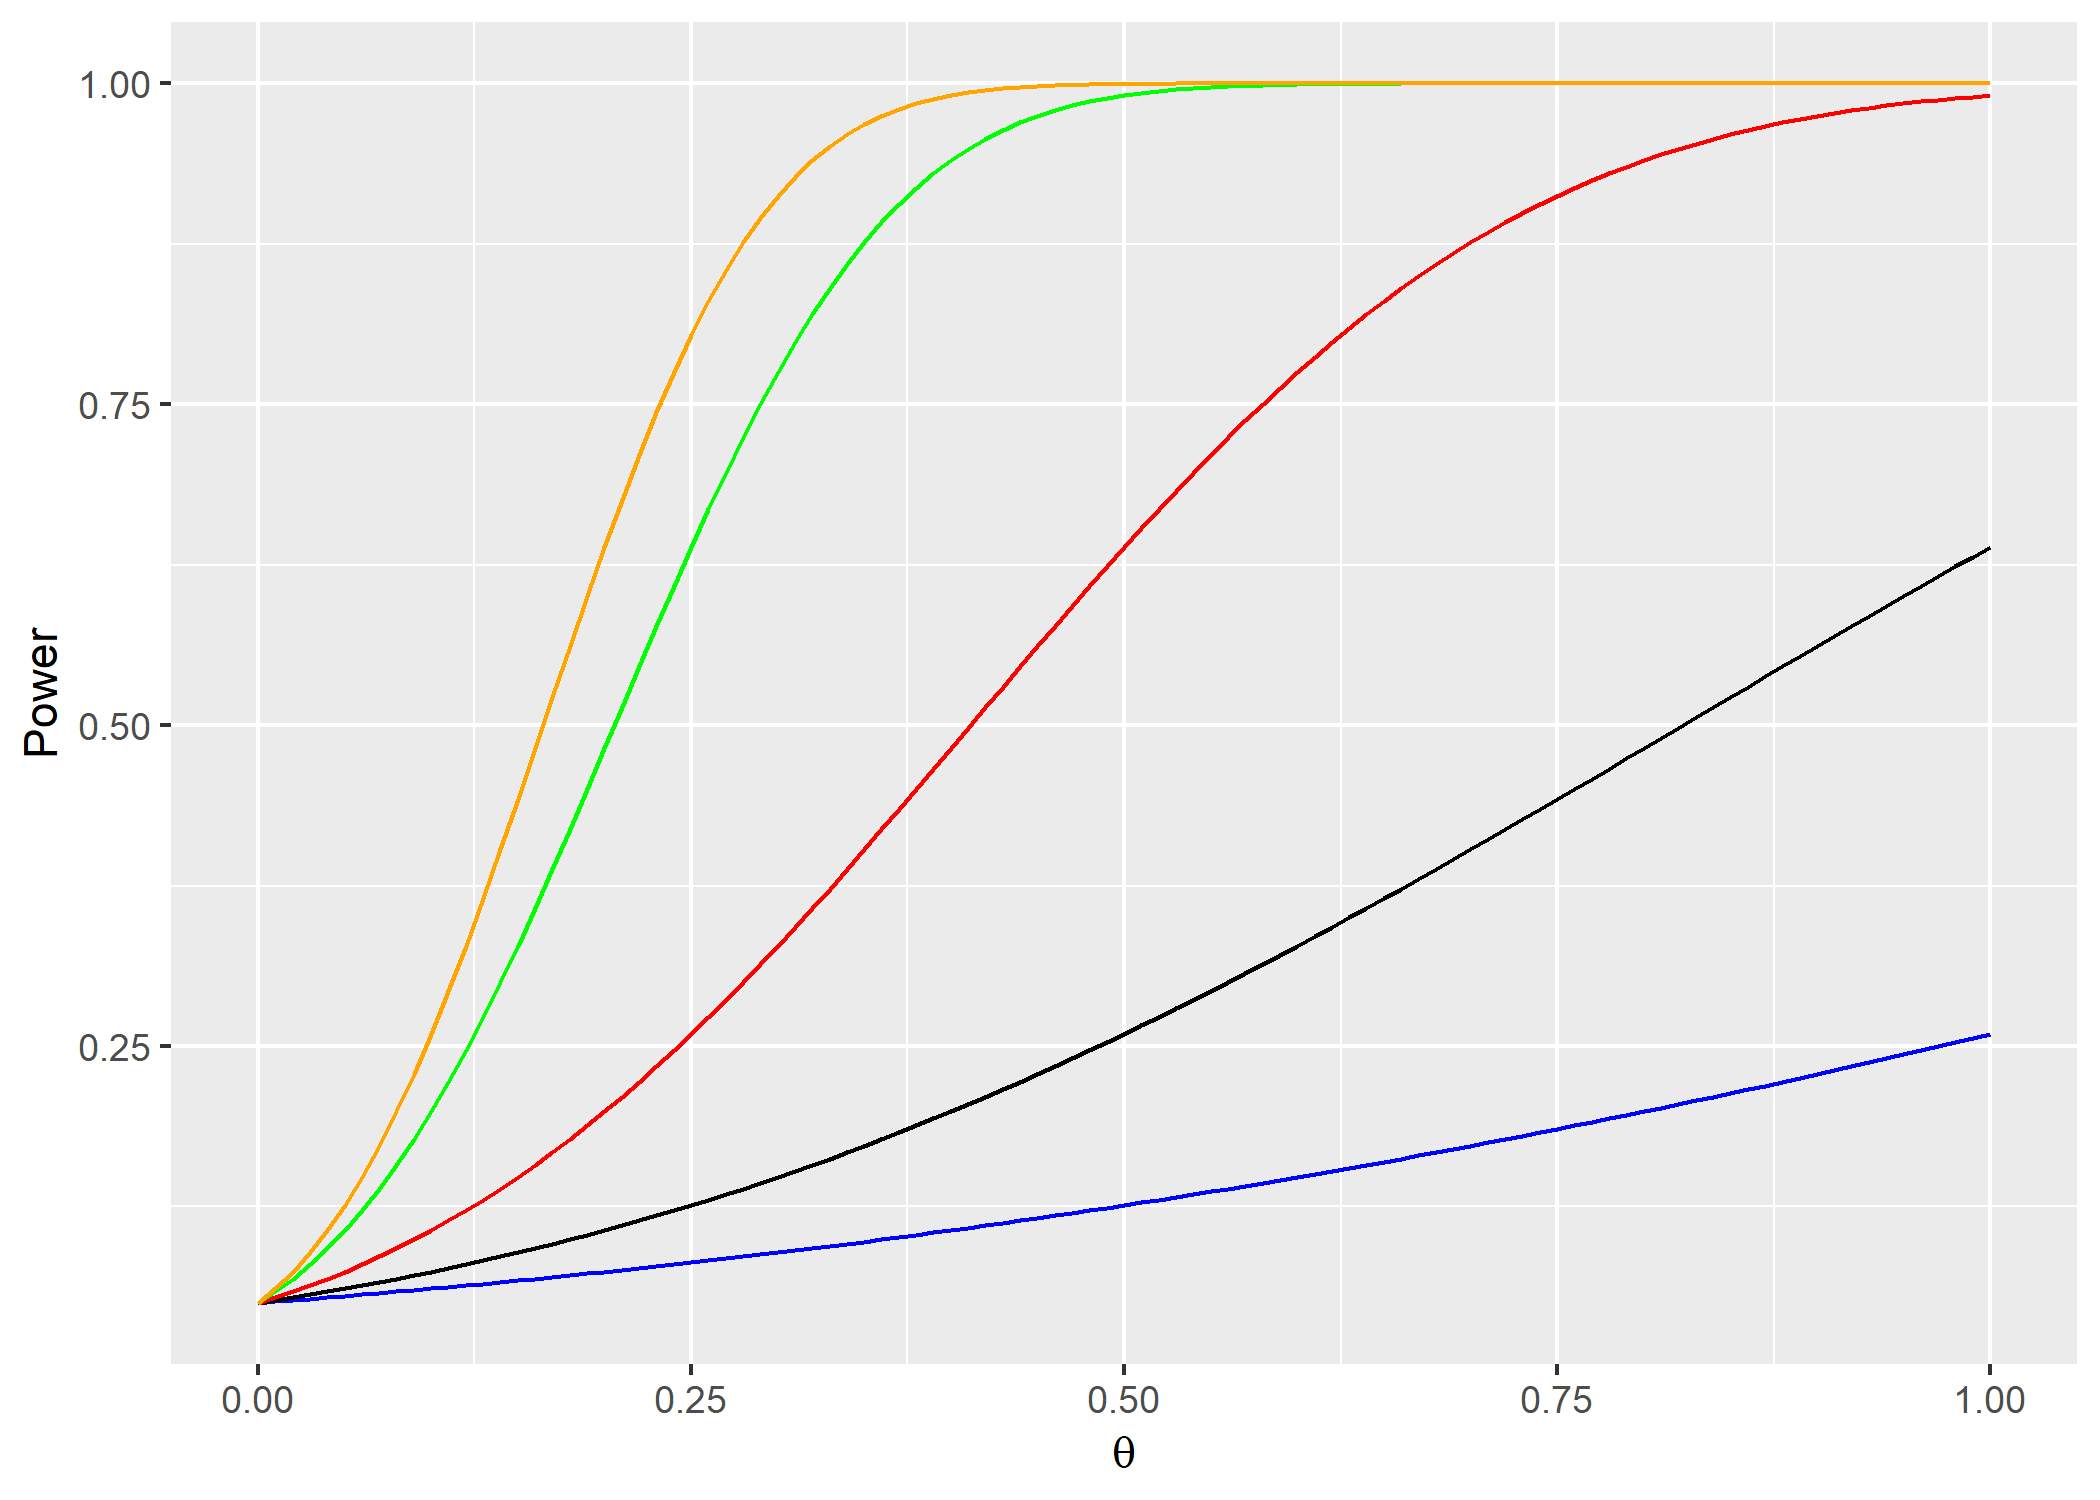
\includegraphics[scale=.7]{Rcode/power1.png}
	\item 
\begin{multline*}\\
H_0:\mu=0 \text{ vs } H_1:\mu\neq 0\\
R=\{\lx<c \}\\
\lra R^*=\{x:\bar{x}\geq c_1^* \text{ or } \leq c_2^*\}\\
\alpha/2=.025=P\left(\dfrac{\bar{X}-\mu_0}{\sg/\sqrt{n}}\geq c^*\right)\\
.025=1-P(Z<c^*)\Rightarrow .975=P(Z<c^*)\\
c^*=qnorm(.975)=1.96\\
-c^*=qnorm(1-.975)=-1.96\\
\B(\mu)=P\left(-c^*\leq\dfrac{\bar{X}-\mu_0}{\sg/\sqrt{n}}\leq c^*\right)\\
=P\left(-1.96\leq\dfrac{\bar{X}-\mu_0}{\sg/\sqrt{n}}\leq 1.96\right)\\
\B(\mu)=P(-1.96-\sqrt{n}\mu/\sg\leq Z\leq 1.96+\sqrt{n}\mu /\sg)\\
Power=.5 \text{ if } \mu=\pm 1.96\sg/\sqrt{n}\\
\end{multline*}
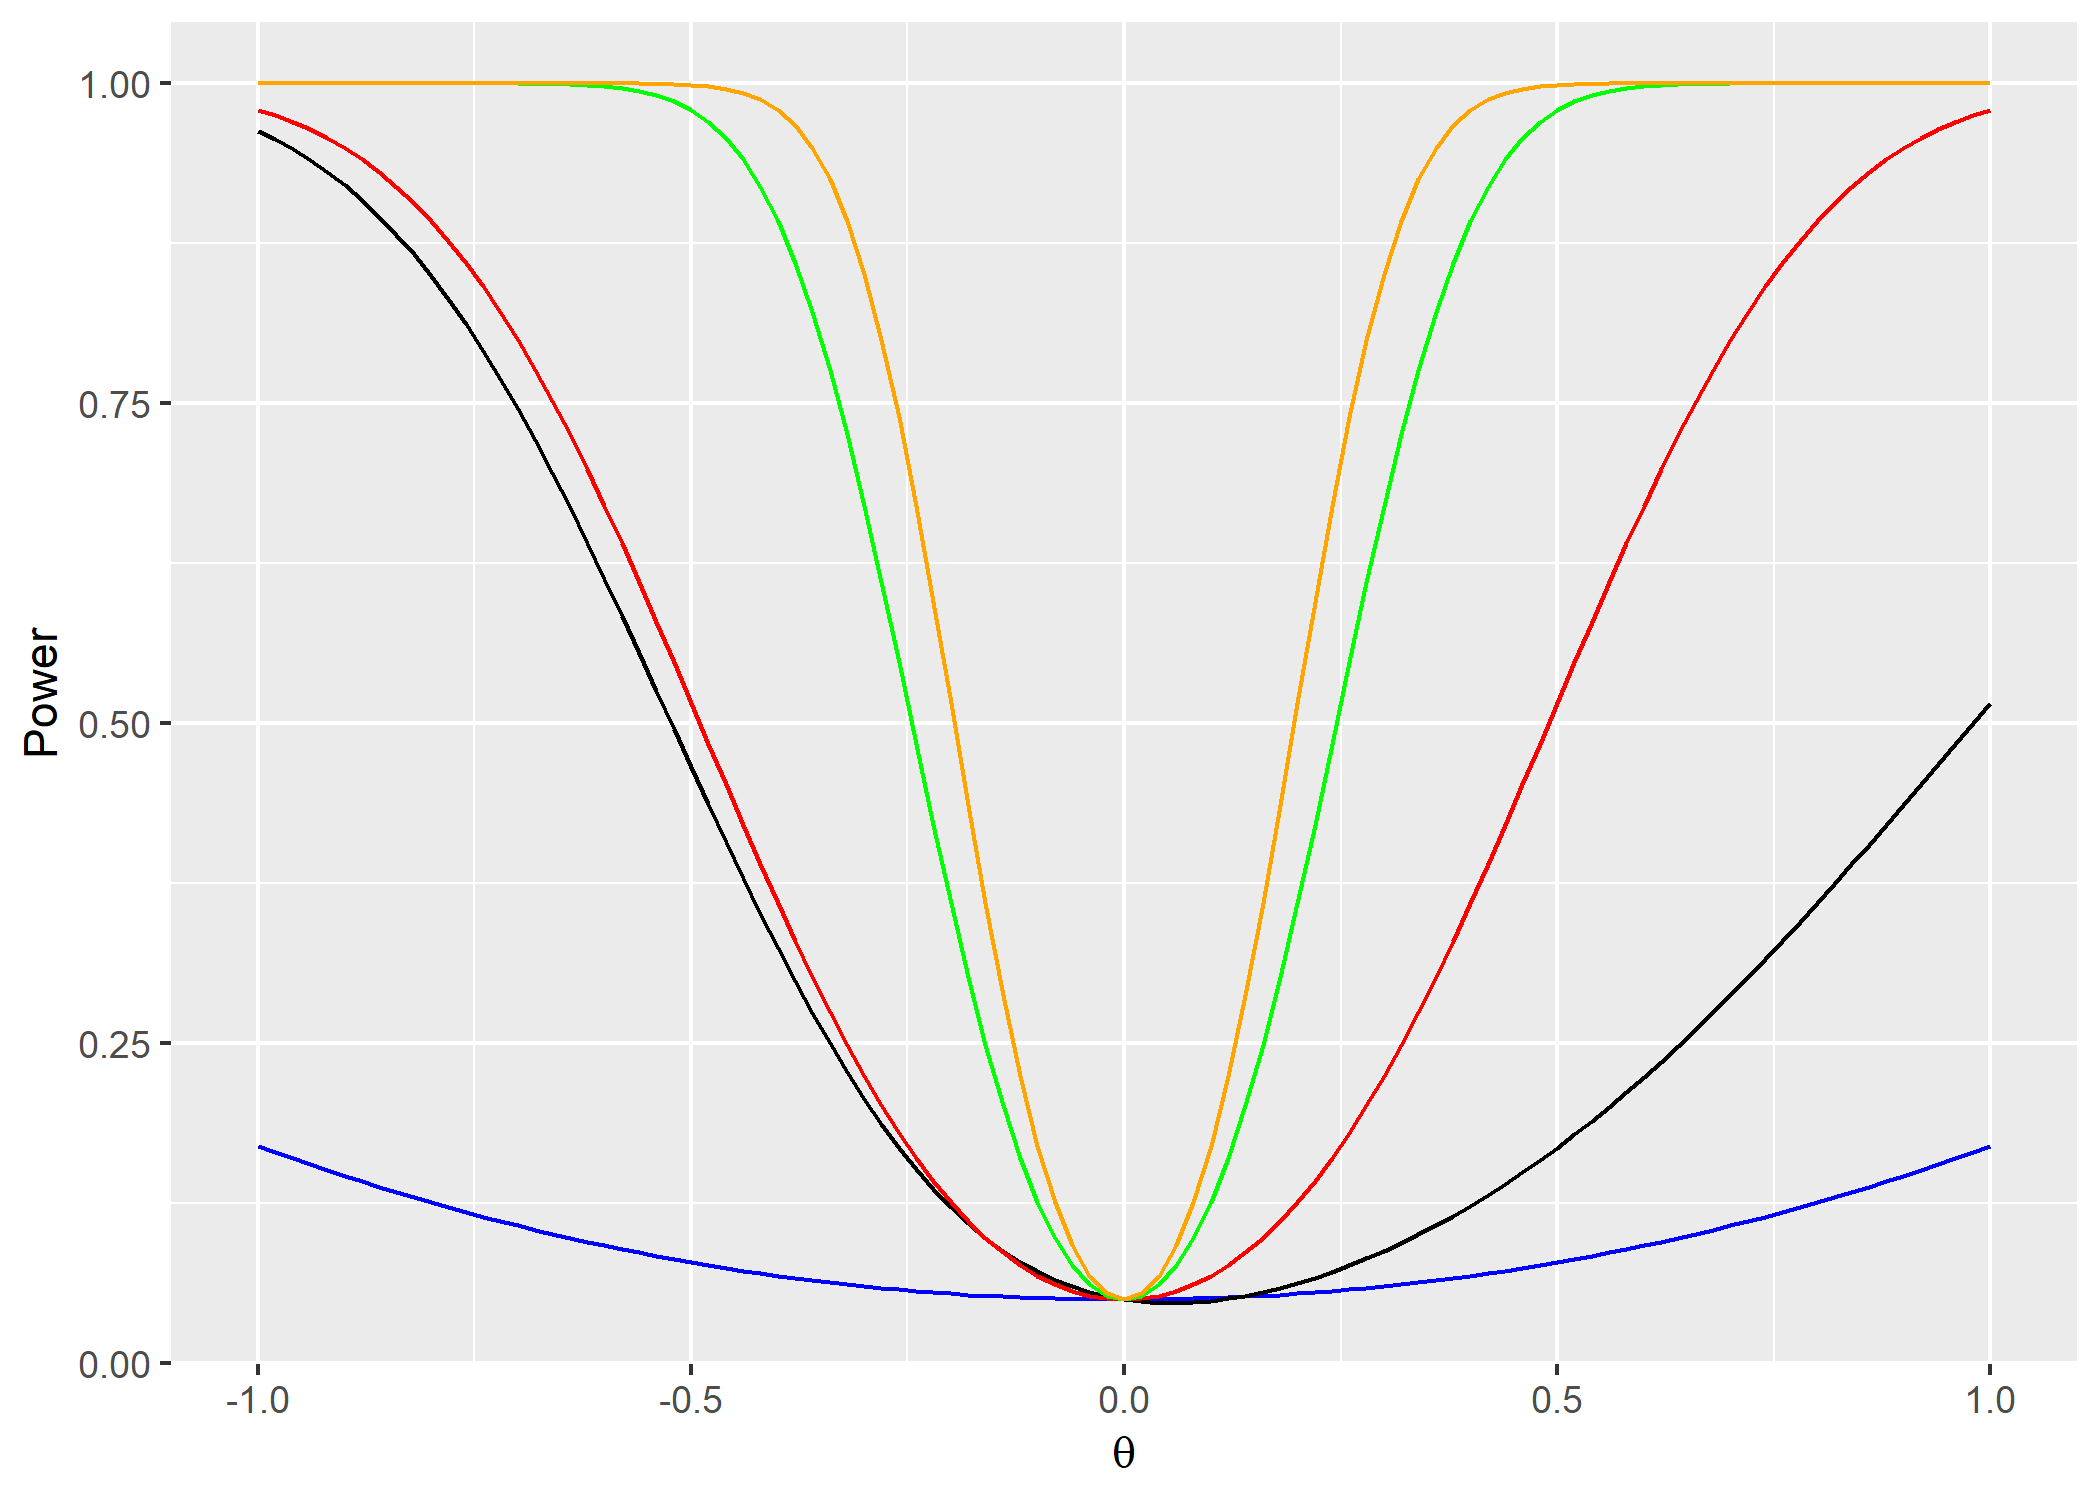
\includegraphics[scale=.7]{Rcode/power2.png}
\end{enumerate}

\section*{Problem 2}

\begin{multline*}\\
\samp f(x|\ta,\lambda)=\dfrac{1}{\lambda}e^{-(x-\ta)/\lambda}I_{[\ta,\infty)}(x)\\
H_0: \ta \leq 0 \text{ vs } H_1:\ta >0\\
L(\ta,\lm|x)=\prodn \dfrac{1}{\lambda}e^{-(x_i-\ta)/\lambda}I_{[\ta,\infty)}(x_i)\\
L(\ta,\lm|x)=\lm^{-n}\exp\left(-(\sumx-n\ta)/\lm \right)I_{[\ta,\infty)}(x_{(1)})\\
L(\ta,\lm|x) \text{ is an increasing function of } \ta\text{ if } \xm \geq \ta  \text{ for any } \lm\\
\mle=\xm\\
\ell=-n\log(\lm)-\dfrac{\sumx-n\hth}{\lm}\\
\pderiv{\ell}{\lm}=\dfrac{-n}{\lm}+\dfrac{\sumx-n\hth}{\lm^2}=0\\
\lm=\dfrac{\sumx-n\hth}{n}=\\
\hat{\lm}=\bar{x}-\hth=\bar{x}-\xm\\
\pderiv{\ell^2}{\lm^2}=\dfrac{n}{\lm^2}-2\dfrac{\sumx-n\hth}{\lm^3}\\
=\dfrac{n}{(\bar{x}-\xm)^2}-2n\left(\dfrac{\bar{x}-\xm}{(\bar{x}-\xm)^3}\right)\\
\pderiv{\ell^2}{\lm^2}=-\left(\dfrac{n}{(\bar{x}-\xm)^2}\right)<0\\
\text{Thus } \hth=\xm, \ \hat{\lm}=\bar{x}-\xm \text{ are the unrestricted MLEs}\\
\text{Under } H_0: \ta\leq 0\\
\hth_0=\begin{cases}
0 & \text{ if } \xm >0\\
\xm & \text{if } \xm \leq 0\\
\end{cases}\\
\text{ For } \xm>0, \ \hth_0=0 \text{ we have:}\\
\ell=-n\log(\lm)-\dfrac{n\bar{x}}{\lm}\\
\pderiv{\ell}{\lm}=-\dfrac{n}{\lm}+\dfrac{n\bar{x}}{\lm^2}=0\\
\hat{\lm}_0=\bar{x}\\
\lx=\dfrac{\sup_{\Theta_0}L(\ta,\lm|x)}{\sup_{\Theta}L(\ta,\lm|x)}=\begin{cases}
1 & \text{ if } \xm\leq 0\\
 \dfrac{L(\ta_0,\lm_0|x)}{L(\hth,\hat{\lm}|x)} & \text{ if } \xm> 0
\end{cases}\\
 \dfrac{L(\ta_0,\lm_0|x)}{L(\hth,\hat{\lm}|x)}=\dfrac{\bar{x}^{-n}\exp\left(-(\sumx-n*0))/\bar{x} \right)}{(\bar{x}-\xm)^{-n}\exp\left(-(\sumx-n\xm)/(\bar{x}-\xm) \right)}\\
=\left(\dfrac{\bar{x}-\xm}{\bar{x}}\right)^n\exp\left(-n-\dfrac{-n(\bar{x}-\xm)}{\bar{x}-\xm}\right)\\
\dfrac{L(\ta_0,\lm_0|x)}{L(\hth,\hat{\lm}|x)}=(1-\xm/\bar{x})^n\\
\lx=\begin{cases}
1 & \text{ if } \xm\leq 0\\
(1-\xm/\bar{x})^n & \text{ if } \xm> 0
\end{cases}\\
T(X)=\xm/\bar{x}\\
\text{ for } \xm > 0,  \ \lx \text{ is a montone increasing function of } T(X) \text{ for every } \bar{x}>\xm\\
\text{Thus the MLR property holds}\\
R=\{x:(1-\xm/\bar{x})^n\leq c \}\\
R=\{x:n\log(1-\xm/\bar{x})\leq \log(c) \}\\
R=\{x:\exp(\log(1-\xm/\bar{x}))\leq \exp(\log(c)/n) \}\\
R=\{x:-\xm/\bar{x}\leq \exp(\log(c)/n)-1 \}\\
R=\{x:\xm/\bar{x}\geq 1-c^{1/n}\}\\
\text{Thus the rejection region is }
R^*=\{x: \xm/\bar{x}\geq c^* \} \quad c^*=1-c^{1/n}\\
\end{multline*}

\section*{Problem 3}
	
\begin{multline*}\\
\samp N(0,\sg^2)\\
H_0:\sg=\sg_0 \text{ vs } H_1:\sg=\sg_1\\
\sg_0<\sg_1\\
L(x|\sg^2)=(2\pi)^{-n/2}(\sg^2)^{-n/2}\exp \left(\dfrac{-\sumx^2}{2\sg^2}\right)\\
\ell(x|\sg^2)\propto (-n/2)\log(\sg^2)-\dfrac{\sumx^2}{2\sg^2}\\
\dll{\sg^2}=(1/2)\left(-\dfrac{n}{\sg^2}+\dfrac{\sumx^2}{\sn^2}\right)=0\\
\hat{\sg^2}_{MLE}=\dfrac{\sumx^2}{n}\\
\dll{\sn^2}^2(\hat{\sg^2})=\dfrac{n}{2\hat{\sn}^2}-\dfrac{\sumx^2}{\hat{\sn}^3}\\
=\dfrac{n/2}{(\sumx^2/n)^2}-\dfrac{\sumx^2}{(\dfrac{\sumx^2}{n})^3}\\
=\dfrac{n/2-n}{(\sumx^2/n)^2}=\dfrac{-n/2}{(\sumx^2/n)^2}<0\\
\text{Thus } \hat{\sg^2}=\dfrac{\sumx^2}{n} \text{ is the unrestricted MLE}\\
\text{Since we have simple vs composite}\\
\text{We can use (N-P) Lemma to construct a UMP level } \alpha \text{ test}\\
R=\{x:\dfrac{f(x|\sg_1)}{f(x|\sg_0)}>c\}\\
\dfrac{f(x|\sg_1)}{f(x|\sg_0)}=\left(\dfrac{2\pi\sg_1^2}{2\pi\sg_0^2}\right)^{-n/2}\dfrac{\exp\left(-\sumn x_i^2/2\sg_1^2\right)}{\exp\left(-\sumn x_i^2 /2\sg_0^2 \right)}\\
=\left(\dfrac{\sg_0}{\sg_1}\right)^n\exp\left(\dfrac{1}{2}\sumn x_i^2(1/\sg_0^2-1/\sg_1^2)\right)\\
R=\{x:\sumn x_i^2>\dfrac{2\log(c(\sg_0/\sg_1)^n)}{(1/\sg_0^2-1/\sg_1^2)} \}\\
c^*=\dfrac{2\log(c(\sg_0/\sg_1)^n)}{(1/\sg_0^2-1/\sg_1^2)}\\
R=\{x:\sumn x_i^2>c^*\}\\
\alpha=P(\sumn x_i^2>c^*)\\
\sumn X_i^2/\sg_0^2\sim \chi_n^2\\
\alpha=P(\sumn X_i^2/\sg_0^2>c^*/\sg_0^2)=P(\chi_n^2>c^*/\sg_0^2)\\
c^*/\sg_0^2=\chi_{n,\alpha}^2\\
c^*=\sg_0^2\chi_{n,\alpha}^2\\
\end{multline*}   

\section*{Problem 4}
	
\begin{enumerate}[(a)]
	
	\item 	
\begin{multline*}\\
f(x|\ta)=(1-\ta)+\dfrac{\ta}{2\sqrt{x}} \quad 0<x<1, \ 0\leq \ta \leq 1\\
f(x|\ta)=\begin{cases}
1  &\text{ if } \ta=0\\
\dfrac{1}{2\sqrt{x}} &\text{ if } \ta=1
\end{cases}\\
R=\{x:\dfrac{f(x|\ta=1)}{f(x|\ta=0)}>c\}\\
\dfrac{f(x|\ta=1)}{f(x|\ta=0)}=\dfrac{\prodn (2\sqrt{x_i})^{-1}}{\prodn 1}\\
=\dfrac{1}{2^n \prodn x_i^{1/2}}\\
R=\{x:\dfrac{1}{2^n \prodn x_i^{1/2}}>c\}\\
=\{x:-n\log(2)-\dfrac{1}{2}\sumn \log(x_i)>\log(c)\}\\
=\{x:-\sumn \log(x_i)>2(\log(c)+n\log(2))\}\\
R=\{x:-\sumn \log(x_i)>c^*\}\\
c^*=2(\log(c)+n\log(2))\\
\text{Let } Y_i=-\log(x_i)\\
e^{-y_i}=x_i\\
J=|-e^{-y_i}|\\
f_{y_i}(y)=f_{x_i}(e^{-y_i})|e^{-y_i}|\\
\text{Since } \ta=0 \quad f_{x_i}(e^{-y_i})=1\\
f_{y_i}(y)=1e^{-y_i}=e^{-y_i} \quad 0<y_i<\infty\\
Y_i\sim Exp(1)\\
\sumn y_i \sim gamma(n,1)\\
\alpha=P(-\sumn log(x_i)>c^*|\ta=0)\\
c^*=gamma(n,1,1-\alpha)\\
R=\{x:-\sumn \log(x_i)>gamma(n,1,1-\alpha) \}\\
\end{multline*}

	\item 
\begin{multline*}\\
n=5 \quad \alpha=.01\\
R=\{x:-\sumn \log(x_i)>gamma(5,1,.99) \}\\
qgamma(p=.99,shape = 5,scale = 1)=11.6\\
R=\{x:-\sumn \log(x_i)>11.6\}\\
Power=P(-\sumn \log(x_i)>11.6|\ta=1)\\
Y_i=-\log(x_i)\\
e^{-y_i}=x_i\\
J=|-e^{-y_i}|\\
f_{y_i}(y)=f_{x_i}(e^{-y_i})|e^{-y_i}|\\
\text{Since } \ta=1 \quad f_{x_i}(e^{-y_i})=\dfrac{1}{2\sqrt{e^{-y_i}}}\\
f_{y_i}(y)=\dfrac{1}{2\sqrt{e^{-y_i}}}e^{-y_i}=\dfrac{1}{2}e^{-y_i/2}\\
Y_i\sim Exp(2)\\
\sumn Y_i \sim gamma(n,2)\\
\text{Since } n=5 \quad\sumn Y_i \sim gamma(5,2)\\
Power=P(-\sum_{i=1}^{5} \log(x_i)>11.6|\ta=1)\\
Power=pgamma(q = 11.6,shape = 5,scale = 2)=.6872817\approx .69\\
\end{multline*}

	\item 
\begin{multline*}\\
P(TypeIError)=.01 \quad P(TypeIIError)=.01\\
Power=1-.01=.99\\
.99=P(-\sumn \log(x_i)>gamma(n,1,.99)|\ta=1)\\
-\sumn \log(x_i)\sim gamma(n,2)\\
\text{Using R, testing } n=1:55 \text{ into}\\
1-pgamma(shape=n,scale=2,q=qgamma(shape=n,scale=1,p=.99))\\
n=45 \ p=0.9891953 \quad n=46 \ p=0.9904418\\
\text{Thus sample size needed is } 46\\
\text{Finding approximate sample size}\\
P(-\sumn \log(x_i)>gamma(n,1,.99)|\ta=1)\\
CLT: \sqrt{n}(\bar{Y}-E(Y_1))\cd N(0,Var(Y_1))\\
.99\approx P(\sumn Y_i>Gamma(n,1,.99)|\ta=1)\\
.99=P(\dfrac{\sqrt{n}(\bar{Y}-E(Y_1))}{\sqrt{Var(Y_1)}}>\dfrac{\sqrt{n}Gamma(n,1,.99)/n)-2}{\sqrt{Var(Y_1)}})\\
\sqrt{Var(Y_1)}=\sqrt{4}=2 \quad E(Y_1)=2\\
P(\sqrt{n}(\bar{Y}-2)/2)>[\sqrt{n}gamma(n,1,.99)/(n)-2]/2)=.99\\
\text{Let } Z=\sqrt{n}(\bar{Y}-2)/2\sim N(0,1)\\
P(Z>(\sqrt{n}gamma(n,1,.99)/(n)-2)/2)=.99\\
1-P(Z\leq(\sqrt{n}gamma(n,1,.99)/(n)-2)/2)=.99\\
P(Z\leq(\sqrt{n}gamma(n,1,.99)/(n)-2)/2)=.01\\
qnorm(.01)=-2.33\\
\sqrt{n}gamma(n,1,.99)/(n)-2)/2=-2.33\\
\text{Using R to Solve:}\\ sqrt(n)*(qgamma(shape=n,scale=1,p=.99)/(n)-2)/2=-2.33\\
\text{We get } n\approx 52\\
\end{multline*}

	\item 
\begin{multline*}\\
f(x|\ta)=(1-\ta)+\dfrac{\ta}{2\sqrt{x}}\\
L^{\prime}(\ta)=-1+\dfrac{1}{2\sqrt{x}}\\
\text{ if } L^{\prime}(\ta)>0 \text{ then } \hth=1\\
\text{ if } L^{\prime}(\ta)<0 \text{ then } \hth=0\\
\text{ if } L^{\prime}(\ta)=0 \text{ then } 0\leq\hth\leq 1\\
-1+\dfrac{1}{2\sqrt{x}}=0\\
2\sqrt{x}=1\\
x=1/4\\
\hth=\begin{cases}
1 & \text{ if } 0<x\leq 1/4\\
0 & \text{ if } 1/4<x<1
\end{cases}\\
E(\hth)=1*P(X\leq 1/4)+0*P(X>1/4)\\
E(\hth)=\int_{0}^{1/4}1(1-\ta+\dfrac{\ta}{2\sqrt{x}})\dx\\
=\bigg |_{0}^{1/4} (1-\ta) x+\ta x^{1/2}=(1-\ta)(1/4)+(1/2)\ta=(1/4)(\ta+1)\\
E(\hth)=(1/4)(\ta+1) \text{ (biased)}\\
E(4\hth-1)=\ta \text{ (unbiased)}\\
T(X_1)=a+b\hth=-1+4\hth\\
\text{The problem with } T(X_1) \text{ as an estimator of } \ta \text{ is:}\\
\hth=0 \Rightarrow T(X_1)=4(0)-1=-1\\
\hth=1 \Rightarrow T(X_1)=4(1)-1=3\\
\text{Neither of these results make sense because}\\
\text{they are outside of the parameter space } 0\leq \ta\leq 1\\
\end{multline*}

\end{enumerate}

	\section*{Problem 5}
\begin{enumerate}[(a)]
	
	\item 
\begin{multline*}\\
Y_i\sim Pois(\ta x_i)\\
f(y|\ta)=\prodn f(y_i|\ta)=\prodn \dfrac{(\ta x_i)^{y_i}e^{-\ta x_i}}{y_i!}\\
=\left(\prodn\dfrac{x_i^{y_i}}{y_i!}\right)\ta^{\sumn y_i}e^{-\ta \sumx}\\
H_0:\ta=1 \text{ vs } \quad H_1:\ta>1\\
\text{Since we have simple vs composite}\\
\text{We can use (N-P) Lemma, to construct a UMP level } \alpha \text{ test}\\
R=\{y:\dfrac{f(y|\ta)}{f(y|\ta=1)}>c\}\\
\dfrac{f(y|\ta)}{f(y|\ta=1)}=\dfrac{\left(\prodn\dfrac{x_i^{y_i}}{y_i!}\right)\te^{\sumn y_i}e^{-\te \sumx}}{\left(\prodn\dfrac{x_i^{y_i}}{y_i!}\right)1^{\sumn y_i}e^{- \sumx}}\\
=\dfrac{\te^{\sumn y_i}e^{-\te \sumx}}{e^{-\sumx}}\\
R=\{y:\te^{\sumn y_i}e^{-\sumx (\te-1)}>c\}\\
\alpha=\sup_{\ta \in H_0}P(\te^{\sumn y_i}e^{-\sumx (\te-1)}>c)\\
\alpha=P_{\ta=1}(\te^{\sumn y_i}e^{-\sumx (\te-1)}>c)\\
R\lra R^*= \{y:T(y)\geq c_1^* \text{or} \leq c_2^* \} \text{ (MLR property)}\\
T(y)=\sumn y_i\\
\{y:\sumn y_i\geq c_1^* \text{or} \leq c_2^* \}\\
R^*=\{y:\sumn y_i \geq c_1^* \} \text{ (R follows the direction of } H_1)\\
\alpha=P(\sumn y_i\geq c_1^*|\ta=1)\\
\sumn y_i\sim Pois(\ta\sumx) =Pois(\sumx) \text{ (since } \ta=1)\\
\end{multline*}

	\item 
\begin{multline*}\\
H_0:\ta\leq 1 \text{ vs } H_1:\ta>1\\
\text{Since we have composite vs composite}\\
\text{We can use (K-R) Theorem, to construct a UMP level } \alpha \text{ test}\\
f(y|\ta)=\left(\prodn\dfrac{x_i^{y_i}}{y_i!}\right)\ta^{\sumn y_i}e^{-\ta \sumx}\\
\dfrac{f(y|\te)}{f(y|\ta_0)} \text{ increasing function of } T(y) \text{ if } \te>\ta_0 \text{ (MLR)}\\
T(y)=\sumn y_i\\
\dfrac{f(y|\te)}{f(y|\ta_0)}=\dfrac{\left(\prodn\dfrac{x_i^{y_i}}{y_i!}\right)\te^{\sumn y_i}e^{-\te \sumx}}{\left(\prodn\dfrac{x_i^{y_i}}{y_i!}\right)\ta_0^{\sumn y_i}e^{- \ta_0\sumx}}\\
\dfrac{f(y|\te)}{f(y|\ta_0)}=\dfrac{\te}{\ta_0}e^{-(\ta_1-\ta_0)\sumx}\\
\ta_1>\ta_0\Rightarrow \dfrac{\te}{\ta_0}>0 \Rightarrow \dfrac{f(y|\te)}{f(y|\ta_0)} \text{ is an increasing function of } \sumn y_i\\ 
R=\{y:\sumn y_i \geq c_1^*\}\\
c_1^*=3 \text{ (from part a)}\\
\end{multline*}

	\item 
\begin{multline*}\\
\sumn y_i\sim Pois(\sumx)=Pois(.8)\\
\alpha=.05=P(\sumn y_i\geq c_1^*|\ta=1)\\
.05=1-P(\sumn y_i<c_1^*)\\
.05=1-P(\sumn y_i\leq c_1^*-1)\\
P(\sumn y_i\leq c_1^*-1)=.95\\
P(X\leq 2)=.952 \quad X\sim Pois(.8)\\
P(\sumn y_i\leq c_1^*-1)\approx P(X\leq 2)\\
\text{Thus } c_1^*=3\\
1-P(\sumn y_i\leq 3-1)=1-.952= .048\\
\end{multline*}

	\item 
\begin{multline*}\\
\sumn y_i \sim Pois(\theta \sumx)=Pois(5*.8)=Pois(4)\\
Power=P(\sumn y_i\geq 3|\ta=5)\\
=1-P(\sumn y_i <3)\\
=1-P(\sumn y_i \leq 2)\\
P(X\leq 2)=.238 \quad X\sim Pois(4)\\
=1-P(\sumn y_i \leq 2)\approx 1-P(X\leq 2)\\
=1-.238=.762\\
Power=.762\\
\end{multline*}
	
\end{enumerate}

\end{flushleft}
\end{document}
